% !TEX TS-program = pdflatex
\documentclass[aspectratio=169]{beamer}
\usepackage[utf8]{inputenc}
\usepackage[T1]{fontenc}
\usetheme{Madrid}
\usecolortheme{seahorse}
\usefonttheme{professionalfonts}
\setbeamertemplate{navigation symbols}{}
\setbeamercovered{transparent}
\setbeamertemplate{itemize items}[circle]
\setbeamertemplate{enumerate items}[default]
\setlength{\parskip}{0.15em}

\definecolor{bepurple}{RGB}{107,63,160}
\definecolor{begold}{RGB}{200,168,75}
\definecolor{beteal}{RGB}{26,122,110}
\definecolor{berust}{RGB}{192,68,42}
\definecolor{beblue}{RGB}{26,74,138}
\definecolor{softpurple}{RGB}{240,232,255}
\definecolor{softgold}{RGB}{255,248,220}
\definecolor{softteal}{RGB}{220,242,240}
\definecolor{softrust}{RGB}{255,235,230}
\setbeamercolor{structure}{fg=beblue}
\setbeamercolor{title}{fg=white,bg=beblue}
\setbeamercolor{frametitle}{fg=beblue}
% Minimal block rendering: regular/example blocks become colored headings (no box)
\setbeamertemplate{block begin}{%
  \par\vspace{0.2ex}%
  \ifx\insertblocktitle\empty\else%
    {\usebeamerfont{block title}\color{beblue}\textbf{\insertblocktitle}}\par\vspace{0.2ex}%
  \fi%
}
\setbeamertemplate{block end}{\par\vspace{0.2ex}}
\setbeamertemplate{block example begin}{%
  \par\vspace{0.2ex}%
  \ifx\insertblocktitle\empty\else%
    {\usebeamerfont{block title}\color{beteal}\textbf{\insertblocktitle}}\par\vspace{0.2ex}%
  \fi%
}
\setbeamertemplate{block example end}{\par\vspace{0.2ex}}
\setbeamertemplate{block alerted begin}{%
  \par\vspace{0.5ex}%
  \begin{beamercolorbox}[sep=0.5ex,rounded=true,shadow=false]{block title alerted}%
    \usebeamerfont{block title}\insertblocktitle%
  \end{beamercolorbox}%
  \nointerlineskip%
  \begin{beamercolorbox}[sep=0.5ex,rounded=true,shadow=false]{block body alerted}%
    \usebeamerfont{block body}%
}
\setbeamertemplate{block alerted end}{\end{beamercolorbox}\par\vspace{0.5ex}}
\setbeamercolor{block title alerted}{fg=white,bg=berust}
\setbeamercolor{block body alerted}{fg=black,bg=berust!8}
\setbeamercolor{alerted text}{fg=berust}

\usepackage{booktabs,amsmath,amssymb,array,multirow,hyperref,colortbl,xcolor}
\usepackage{tikz}
\usepackage{pgfplots}
\pgfplotsset{compat=1.18}
\usetikzlibrary{arrows.meta,positioning,calc,shapes.geometric,patterns,trees}
\hypersetup{colorlinks=true,linkcolor=beblue,urlcolor=beblue}

\title{\textbf{Lecture 2: Heuristics and Biases}}
\subtitle{Mental Shortcuts and Their Systematic Consequences}
\author{Prof.\ Muhebullah Karimzada}
\institute{School of Economics, University of Northern British Columbia}
\date{ECON 230 $\cdot$ Introduction to Behavioural Economics $\cdot$ Winter 2027}

\begin{document}

\begin{frame}[plain]\titlepage\end{frame}

% ============================================================
\begin{frame}{Which Kills More People?}
\note{This opening exercise shocks students because their intuitions are so wrong. The point is that our perception of risk is driven by how easily we can recall examples --- the availability heuristic.}
\begin{alertblock}{Quick Quiz: Which kills more Americans/year? (A or B)}
\small\begin{tabular}{lll}
& \textbf{A} & \textbf{B}\\
\midrule
1. & Shark attacks & Falling out of bed\\
2. & Deer (car collisions) & Lightning strikes\\
3. & Tornadoes & Bee stings\\
4. & Plane crashes & Car crashes (per km)\\
\end{tabular}
\end{alertblock}
\pause
\begin{columns}
\column{0.5\textwidth}
\textcolor{beblue}{\textbf{Answers (CDC):}}\small
\begin{itemize}\itemsep0pt
  \item Bed falls \textbf{450/yr} vs Sharks \textbf{6/yr}
  \item Deer \textbf{130/yr} vs Lightning \textbf{50/yr}
  \item Bee stings \textbf{62/yr} vs Tornadoes \textbf{70/yr}
  \item Cars \textbf{1.37/100M km} vs Planes \textbf{0.07}
\end{itemize}
\column{0.47\textwidth}
\begin{exampleblock}{Why Wrong?}
Sharks, planes, tornadoes: \alert{vivid and memorable}. Bed falls: quiet, no headlines. This is the \textbf{Availability Heuristic}.
\end{exampleblock}
\end{columns}
\end{frame}

% ============================================================
\begin{frame}{Lecture Roadmap}
\begin{block}{Five Heuristics and Biases Today}
\begin{enumerate}
  \item \textbf{Dual Process Theory} --- System 1 vs System 2
  \item \textbf{Representativeness} --- Judge by resemblance (Linda Problem, Base Rate Neglect)
  \item \textbf{Availability} --- Judge by ease of recall (risks, markets)
  \item \textbf{Anchoring} --- Adjust from a starting point (insufficiently)
  \item \textbf{Confirmation Bias} --- Seek confirming evidence
  \item \textbf{Overconfidence} --- Overestimate accuracy and ability
\end{enumerate}
\end{block}
\begin{exampleblock}{Key Message}
These are not random errors. They are \alert{systematic, predictable, and stable across populations}. That is what makes them economically important.
\end{exampleblock}
\end{frame}

% ============================================================
\section{System 1 vs System 2}
% ============================================================

\begin{frame}{Dual Process Theory}
\note{Kahneman's 2011 book 'Thinking, Fast and Slow' synthesises 40 years of research. System 1 is not 'bad' -- it is fast, efficient, and usually correct. The problem arises when System 1 is applied to situations that require System 2 analysis.}
\begin{columns}
\column{0.47\textwidth}
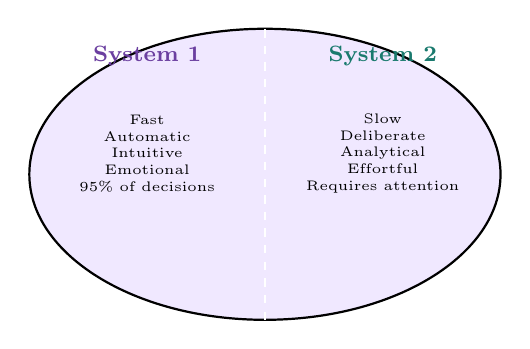
\begin{tikzpicture}[scale=0.88]
\draw[thick,fill=softpurple] (0,0) ellipse (3.4cm and 2.1cm);
\draw[thick,white,dashed] (0,-2.1) -- (0,2.1);
\node[bepurple,font=\bfseries\footnotesize] at (-1.7,1.7) {System 1};
\node[font=\tiny,text width=2.8cm,align=center] at (-1.7,0.3) {Fast \\ Automatic \\ Intuitive \\ Emotional \\ 95\% of decisions};
\node[beteal,font=\bfseries\footnotesize] at (1.7,1.7) {System 2};
\node[font=\tiny,text width=2.8cm,align=center] at (1.7,0.3) {Slow \\ Deliberate \\ Analytical \\ Effortful \\ Requires attention};
\end{tikzpicture}
\column{0.5\textwidth}
\begin{block}{System 1 Examples}
Reading a face, driving a familiar route, $2 \times 2$, catching a ball, speaking your native language.
\end{block}
\begin{block}{System 2 Examples}
Solving $17 \times 24$, navigating a new city, writing an economics essay, following a complex legal argument.
\end{block}
\begin{alertblock}{Kahneman's Key Insight}
System 1 is \textbf{``lazy System 2's'' servant}. System 2 endorses System 1's output without checking --- most of the time.
\end{alertblock}
\end{columns}
\end{frame}

% ============================================================
\begin{frame}{Decision Fatigue --- System 2 Gets Tired}
\begin{columns}
\column{0.52\textwidth}
\begin{exampleblock}{The Israeli Parole Board (Danziger et al., 2011)}
Analysed 1,112 parole board decisions across a full day.
\begin{itemize}
  \item \textbf{Start of session:} 65\% approval rate.
  \item \textbf{Just before food break:} Near \textbf{0\%} approval.
  \item \textbf{After food break:} Back to \textbf{65\%}.
\end{itemize}
\textit{The pattern repeated three times per day.}
\end{exampleblock}
\begin{exampleblock}{Interpretation}
When System 2 is depleted by decision-making, it defaults to the \textbf{safe, status-quo option} (deny parole). The prisoner's fate depended on \textit{when} the hearing was scheduled.
\end{exampleblock}
\column{0.45\textwidth}
\begin{tikzpicture}
\begin{axis}[
  width=\textwidth,height=0.7\textheight,
  xlabel={\small Time of Day},ylabel={\small \% Parole Granted},
  title={\small Israeli Parole Board Study},
  xmin=0,xmax=8,ymin=0,ymax=80,
  xtick={1,3,5,7},
  xticklabels={Morning,Pre-lunch,Afternoon,Pre-end},
  x tick label style={font=\tiny,rotate=20,anchor=east},
  axis lines=left
]
\addplot[beblue,very thick] coordinates{(0.5,65)(2,30)(3,5)(3.5,65)(5,40)(5.5,5)(6,65)(7.5,20)};
\draw[dashed,beteal] (axis cs:3,0) -- (axis cs:3,80) node[above,font=\tiny]{\textit{lunch}};
\draw[dashed,beteal] (axis cs:5.8,0) -- (axis cs:5.8,80) node[above,font=\tiny]{\textit{snack}};
\end{axis}
\end{tikzpicture}
\end{columns}
\end{frame}

% ============================================================
\section{Representativeness Heuristic}
% ============================================================

\begin{frame}{The Representativeness Heuristic}
\begin{block}{Definition (Kahneman \& Tversky, 1972)}
We judge the probability that object $X$ belongs to category $Y$ by how much $X$ \textit{resembles} our mental prototype of $Y$ --- \textbf{ignoring base rates and sample size}.
\end{block}
\begin{columns}
\column{0.5\textwidth}
\begin{exampleblock}{Classic Example}
Tom is a quiet, detail-oriented person who loves puzzles and sci-fi. Is Tom more likely to be a librarian or a truck driver?
\end{exampleblock}
\pause
\column{0.47\textwidth}
\begin{alertblock}{The Answer}
\textbf{Truck driver} --- by far. There are $\approx$3.5 million truck drivers in the US vs $\approx$170,000 librarians. The base rate alone predicts truck driver, even if Tom fits the librarian stereotype perfectly.
\end{alertblock}
\end{columns}
\medskip
Representativeness ignores the \alert{prior probability} (base rate) and focuses on the \alert{likelihood} of the description.
\end{frame}

% ============================================================
\begin{frame}{[GAME] The Linda Problem}
\note{This is the most famous experiment in cognitive psychology. 85-90\% of respondents choose B even when they understand probability theory. Run the show of hands BEFORE revealing the answer.}
\begin{exampleblock}{Linda's Description}
``Linda is 31 years old, single, outspoken, and very bright. She majored in philosophy. As a student, she was deeply concerned with discrimination and social justice, and participated in anti-nuclear demonstrations.''
\end{exampleblock}
\begin{alertblock}{Rank by Probability (write your answer)}
\textbf{A.} Linda is a bank teller.\\[0.3em]
\textbf{B.} Linda is a bank teller and is active in the feminist movement.
\end{alertblock}
\pause
\begin{block}{The Answer: A $\geq$ B. \textit{Always.} By the laws of probability.}
$P(\text{bank teller} \cap \text{feminist}) \leq P(\text{bank teller})$. Yet \textbf{85\%} of subjects chose B (Tversky \& Kahneman, 1983). Replicated in doctors, statisticians, and Nobel Prize winners.
\end{block}
\end{frame}

% ============================================================
\begin{frame}{The Conjunction Fallacy --- A Venn Diagram}
\begin{columns}
\column{0.45\textwidth}
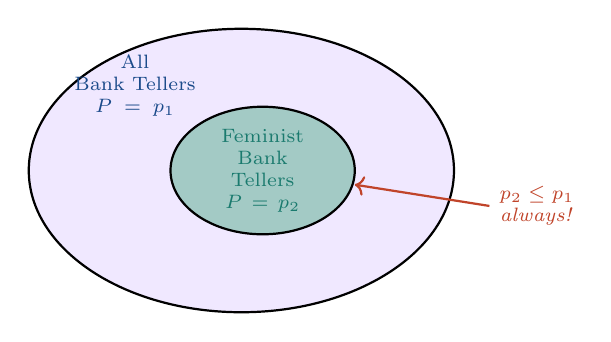
\begin{tikzpicture}[scale=0.9]
\draw[thick,fill=softpurple] (0,0) ellipse (3cm and 2cm);
\draw[thick,fill=beteal!40] (0.3,0) ellipse (1.3cm and 0.9cm);
\node[font=\scriptsize,beblue,text width=2cm,align=center] at (-1.5,1.2) {All\\Bank Tellers\\$P = p_1$};
\node[font=\scriptsize,beteal,text width=1.5cm,align=center] at (0.3,0) {Feminist\\Bank Tellers\\$P = p_2$};
\draw[thick,->,berust] (3.5,-0.5) node[right,font=\scriptsize,berust,align=left]{$p_2 \leq p_1$\\\textit{always!}} -- (1.6,-0.2);
\end{tikzpicture}
\column{0.52\textwidth}
\begin{block}{The Conjunction Rule}
$P(A \cap B) \leq P(A)$ for any events $A$, $B$.\\[0.4em]
Adding conditions can \textbf{only reduce or maintain} probability. It can \textit{never} increase it.
\end{block}
\begin{alertblock}{Why People Violate This}
Linda's description \alert{resembles} a feminist bank teller more than a generic bank teller. Representativeness overrides probability theory.
\end{alertblock}
\begin{exampleblock}{Economic Implication}
Investors believe stories like ``tech stock rises because AI boom AND rate cuts'' is more likely than just ``tech stock rises'' --- leading to overconfidence in complex narratives.
\end{exampleblock}
\end{columns}
\end{frame}

% ============================================================
\begin{frame}{Base Rate Neglect --- Medical Diagnosis}
\begin{columns}
\column{0.5\textwidth}
\begin{block}{The Scenario}
\begin{itemize}
  \item Disease affects \textbf{1 in 1,000} people.
  \item Test is \textbf{99\% accurate} (1\% false positive rate).
  \item You test positive. What is the probability you have the disease?
\end{itemize}
\end{block}
\pause
\begin{alertblock}{Most People Say: $\approx 99\%$. Correct Answer: $\approx 9\%$}
\begin{itemize}
  \item 1,000 people tested: 1 true positive (tests positive), 10 false positives.
  \item $P(\text{disease} | +) = \dfrac{1}{1+10} \approx 9\%$
\end{itemize}
\end{alertblock}
\column{0.47\textwidth}
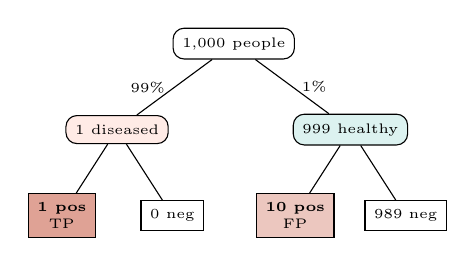
\begin{tikzpicture}[scale=0.78,
  level 1/.style={sibling distance=3.8cm,level distance=1.4cm},
  level 2/.style={sibling distance=1.8cm,level distance=1.4cm},
  every node/.style={font=\tiny},
  edge from parent/.style={draw,thin}]
\node[draw,rounded corners] {1{,}000 people}
  child {node[draw,fill=softrust,rounded corners]{1 diseased}
    child {node[draw,fill=berust!50,align=center]{\textbf{1 pos}\\TP}}
    child {node[draw,align=center]{0 neg}}
    edge from parent node[left]{99\%}
  }
  child {node[draw,fill=softteal,rounded corners]{999 healthy}
    child {node[draw,fill=berust!30,align=center]{\textbf{10 pos}\\FP}}
    child {node[draw,align=center]{989 neg}}
    edge from parent node[right]{1\%}
  };
\end{tikzpicture}
\textcolor{berust}{\textbf{Of 11 positives: only 1 is truly diseased!}}
\end{columns}
\end{frame}

% ============================================================
\begin{frame}{The Gambler's Fallacy}
\begin{columns}
\column{0.5\textwidth}
\begin{block}{Definition}
After a streak (e.g., 5 heads in a row), people believe the opposite is now ``due.'' The random process is expected to \alert{self-correct}.
\end{block}
\textcolor{beteal}{\textbf{Why It Happens:}} HHHHH does not \textit{look} random; HTTHHT does. Representativeness drives expectations.
\begin{alertblock}{Economic Consequences}
\begin{itemize}\small
  \item Casino players bet against streaks at roulette.
  \item Lottery players avoid ``recent'' winning numbers.
  \item Loan officers less likely to approve after approving loan $n-1$ (Rao et al., 2019).
\end{itemize}
\end{alertblock}
\column{0.47\textwidth}
\begin{tikzpicture}
\begin{axis}[
  width=\textwidth,height=0.6\textheight,
  xlabel={\small Number of Heads in a Row},
  ylabel={\small Believed Prob(Next = Tails)},
  xmin=0,xmax=6,ymin=0.4,ymax=0.9,
  axis lines=left,
  title={\small Gambler's Fallacy (Survey Data)}
]
\addplot[berust,very thick] coordinates{(0,0.5)(1,0.52)(2,0.58)(3,0.66)(4,0.75)(5,0.82)};
\addplot[beteal,dashed,thick,domain=0:6]{0.5} node[right,font=\tiny,beteal]{Correct (50\%)};
\end{axis}
\end{tikzpicture}
\end{columns}
\end{frame}

% ============================================================
\section{Availability Heuristic}
% ============================================================

\begin{frame}{The Availability Heuristic}
\begin{block}{Definition (Tversky \& Kahneman, 1973)}
We judge the frequency or probability of events by how \textbf{easily examples come to mind}. Vivid, recent, dramatic events are more available --- and therefore judged more likely.
\end{block}
\begin{columns}
\column{0.5\textwidth}
\begin{block}{Classic Demonstration}
``Are there more English words that start with K, or words with K as the 3rd letter?''
\begin{itemize}
  \item Most say: \textit{start with K}
  \item Correct: \textit{3rd letter} (by a factor of $\approx 3\times$)
  \item It's just much easier to retrieve K-first words.
\end{itemize}
\end{block}
\column{0.47\textwidth}
\begin{tikzpicture}
\begin{axis}[
  width=\textwidth,height=0.6\textheight,
  ybar,bar width=0.6cm,
  ylabel={\small Annual US Deaths},
  symbolic x coords={Sharks,Bed Falls,Tornadoes,Bee Stings},
  xtick=data,
  x tick label style={font=\tiny,rotate=30,anchor=east},
  nodes near coords,
  title={\small Perceived vs Actual Risk (CDC)},
  legend pos=north east
]
\addplot[fill=berust!70] coordinates{(Sharks,100)(Bed Falls,100)(Tornadoes,100)(Bee Stings,100)};
\addplot[fill=beteal!70] coordinates{(Sharks,6)(Bed Falls,450)(Tornadoes,70)(Bee Stings,62)};
\legend{\small Perceived Rank,\small Actual Deaths}
\end{axis}
\end{tikzpicture}
\end{columns}
\end{frame}

% ============================================================
\begin{frame}{Availability Cascade}
\begin{block}{Kuran \& Sunstein (1999)}
An \alert{availability cascade}: a self-reinforcing cycle where:
\begin{enumerate}
  \item A minor risk event occurs.
  \item Media covers it intensively --- it becomes highly available.
  \item Public perceives the risk as much larger.
  \item More media attention follows.
  \item Policy responds to the inflated public fear.
\end{enumerate}
\end{block}
\begin{columns}
\column{0.5\textwidth}
\begin{exampleblock}{Alar Pesticide Scare (1989)}
CBS 60 Minutes reported Alar (used on apples) as ``the most potent cancer-causing agent in the food supply.'' Zero documented deaths. Yet apple sales collapsed 25\% in 3 months. Schools banned apples. Cost to industry: \$375M.
\end{exampleblock}
\column{0.47\textwidth}
\begin{alertblock}{Contrast: Radon in Homes}
Radon kills $\approx$21,000 Americans per year --- 3rd leading cause of lung cancer. Almost no media coverage. Almost no public concern. Low availability = low perceived risk.
\end{alertblock}
\end{columns}
\end{frame}

% ============================================================
\section{Anchoring Heuristic}
% ============================================================

\begin{frame}{The Anchoring Effect}
\begin{block}{Tversky \& Kahneman (1974)}
When making quantitative judgments, people start from an initial value (the \alert{anchor}) and adjust --- but they adjust \textbf{insufficiently}. The final estimate is biased toward the anchor, even if it is \textit{clearly arbitrary}.
\end{block}
\begin{exampleblock}{The Spinning Wheel Experiment}
Tversky \& Kahneman had subjects spin a ``rigged'' wheel that landed on either 10 or 65. They were then asked: ``What \% of African nations are in the UN?''
\begin{itemize}
  \item Wheel landed on 10: mean estimate = \textbf{25\%}
  \item Wheel landed on 65: mean estimate = \textbf{45\%}
  \item The random wheel number shifted answers by \alert{20 percentage points}.
\end{itemize}
\end{exampleblock}
\begin{alertblock}{Why Do Irrelevant Numbers Matter?}
Even when people know the anchor is random, they cannot fully disengage from it. The anchor activates nearby numeric concepts in memory, biasing retrieval.
\end{alertblock}
\end{frame}

% ============================================================
\begin{frame}{[GAME] Anchoring in the Classroom}
\note{Divide the class in half again. This time for anchoring on a price estimate. The point: irrelevant numbers shift real economic estimates. Run this BEFORE discussing the mechanism.}
\begin{columns}
\column{0.48\textwidth}
\begin{block}{Group A --- Left Side}
\begin{enumerate}
  \item Is a bottle of 1998 Bordeaux wine worth \textbf{more or less than \$10}?
  \item Write your \textbf{best estimate} of its value.
\end{enumerate}
\end{block}
\column{0.48\textwidth}
\begin{alertblock}{Group B --- Right Side}
\begin{enumerate}
  \item Is a bottle of 1998 Bordeaux wine worth \textbf{more or less than \$400}?
  \item Write your \textbf{best estimate} of its value.
\end{enumerate}
\end{alertblock}
\end{columns}
\pause
\medskip
\begin{block}{Expected Results (Ariely, Loewenstein \& Prelec, 2003)}
\begin{itemize}
  \item Group A mean: $\approx \$20$--$35$
  \item Group B mean: $\approx \$85$--$130$
  \item \textbf{Neither group can verify the correct price} --- yet the anchor dominates.
  \item Ariely et al.\ called this \alert{``arbitrary coherence''}: once anchored, people are internally consistent but externally anchored.
\end{itemize}
\end{block}
\end{frame}

% ============================================================
\begin{frame}{Anchoring in Real Markets}
\begin{columns}
\column{0.5\textwidth}
\begin{exampleblock}{Real Estate (Northcraft \& Neale, 1987)}
Experienced real estate agents were shown the same property with different listing prices. Their estimated values differed by up to \textbf{11\%}. The listing price anchored even expert valuers.
\end{exampleblock}
\begin{exampleblock}{Salary Negotiation}
Galinsky \& Mussweiler (2001): the first salary offer anchors the final settlement. Making a first offer first --- even a high one --- predicts 10--15\% higher final salary.
\end{exampleblock}
\column{0.47\textwidth}
\begin{exampleblock}{Legal Sentencing (Englich et al., 2006)}
German judges were asked to roll a die before sentencing a shoplifter.
\begin{itemize}
  \item Die rolled 3: recommended sentence = \textbf{5 months}
  \item Die rolled 9: recommended sentence = \textbf{8 months}
\end{itemize}
\alert{A random number shifted prison sentences by 50\%.} Judges knew the die was random.
\end{exampleblock}
\end{columns}
\medskip
\begin{block}{Retail Anchoring}
``Compare at \$200 --- Our price: \$79'' exploits anchoring. The fictitious \$200 anchors perceived value, making \$79 seem like a bargain, regardless of actual market value.
\end{block}
\end{frame}

% ============================================================
\section{Confirmation Bias}
% ============================================================

\begin{frame}{Confirmation Bias}
\begin{block}{Definition}
We search for, interpret, favour, and recall information in a way that \textbf{confirms our pre-existing beliefs}. Disconfirming evidence receives less attention and is more easily dismissed.
\end{block}
\begin{columns}
\column{0.5\textwidth}
\begin{exampleblock}{Wason (1960) Selection Task}
Cards: each has a number on one side and a letter on the other. You see: \textbf{E, K, 4, 7}. Rule: ``If a card has E on one side, it has 4 on the other.'' Which cards must you turn over?
\end{exampleblock}
\pause
\begin{block}{Correct Answer: E and 7}
Most say E and 4. They seek \textit{confirming} cases (E and 4) and ignore the falsifying case (7 with E on the back would violate the rule). Only 10\% solve this correctly.
\end{block}
\column{0.47\textwidth}
\begin{alertblock}{In Financial Markets}
Investors interpret ambiguous earnings news as confirming their existing position.
\begin{itemize}
  \item Bull: ``Inflation fell --- great for growth!''
  \item Bear: ``Inflation fell --- recession signal!''
\end{itemize}
Lord, Ross \& Lepper (1979): subjects who read \textit{the same} mixed evidence study both concluded it \textit{strengthened} their prior views.
\end{alertblock}
\end{columns}
\end{frame}

% ============================================================
\section{Overconfidence}
% ============================================================

\begin{frame}{Three Types of Overconfidence}
\textcolor{beblue}{\textbf{Moore \& Healy (2008) Taxonomy:}}
\begin{enumerate}\small
  \item \textbf{Overprecision:} Your 90\% confidence intervals are too narrow.
  \item \textbf{Overplacement (Better-Than-Average):} You think you perform above your peer group.
  \item \textbf{Overestimation:} You overestimate your absolute ability or performance.
\end{enumerate}
\begin{columns}
\column{0.5\textwidth}
\begin{alertblock}{Key Data}
\begin{itemize}\small
  \item \textbf{93\%} of US drivers: above average (Svenson, 1981)
  \item \textbf{94\%} of professors: above-average teachers (Cross, 1977)
  \item \textbf{84\%} of French drivers: above average
  \item Finance professors: 80\% CI captures actual S\&P return only \textbf{33\%} of the time (Graham \& Harvey, 2003)
\end{itemize}
\end{alertblock}
\column{0.47\textwidth}
\begin{tikzpicture}
\begin{axis}[
  width=\textwidth,height=0.6\textheight,
  xlabel={\small Actual Skill Percentile},
  ylabel={\small Perceived Skill Percentile},
  xmin=0,xmax=100,ymin=0,ymax=100,
  axis lines=left,
  title={\small Better-Than-Average Effect}
]
\addplot[black,dashed,domain=0:100]{x};
\addplot[berust,thick,domain=0:100]{30+0.4*x};
\node[font=\tiny,black,rotate=40] at (axis cs:70,75) {Perfect calibration};
\node[font=\tiny,berust,rotate=22] at (axis cs:70,57) {Actual ratings};
\end{axis}
\end{tikzpicture}
\end{columns}
\end{frame}

% ============================================================
\begin{frame}{The Dunning-Kruger Effect}
\begin{columns}
\column{0.5\textwidth}
\begin{block}{Kruger \& Dunning (1999)}
Low-competence individuals most severely overestimate their ability. High-competence individuals slightly underestimate.
\end{block}
\begin{quote}
\textit{``The trouble with the world is that the stupid are cocksure and the intelligent are full of doubt.''}\\--- Bertrand Russell
\end{quote}
\begin{exampleblock}{Application}
Entry-level managers who don't know what they don't know. New investors who made money in a bull market. First-year students who haven't encountered hard questions yet.
\end{exampleblock}
\column{0.47\textwidth}
\begin{tikzpicture}
\begin{axis}[
  width=\textwidth,height=0.65\textheight,
  xlabel={\small Actual Competence},
  ylabel={\small Perceived Competence},
  xmin=0,xmax=10,ymin=0,ymax=10,
  title={\small Dunning-Kruger Curve},
  axis lines=left
]
\addplot[black,dashed,domain=0:10]{x};
\addplot[bepurple,very thick] coordinates{(0,6)(2,8)(3,8.5)(4,7)(6,6)(8,7.5)(10,9.5)};
\node[font=\tiny,black,rotate=40] at (axis cs:7,7.8) {Perfect calibration};
\node[font=\tiny,bepurple] at (axis cs:2,9){\textbf{``Mount Stupid''}};
\node[font=\tiny,bepurple] at (axis cs:4.5,5.5){\textit{Valley of Despair}};
\node[font=\tiny,bepurple] at (axis cs:9,8.2){\textit{Mastery}};
\end{axis}
\end{tikzpicture}
\end{columns}
\end{frame}

% ============================================================
\begin{frame}{Overconfidence and Financial Markets}
\begin{columns}
\column{0.5\textwidth}
\begin{alertblock}{Barber \& Odean (2001) --- ``Boys Will Be Boys''}
\begin{itemize}\small
  \item Men trade \textbf{45\% more}; net returns \textbf{1.4\% lower} than buy-and-hold.
  \item Women trade less; net returns \textbf{0.94\% lower}. Both lose to inaction.
  \item Overconfidence $\Rightarrow$ excess trading $\Rightarrow$ destroyed returns.
\end{itemize}
\end{alertblock}
\textcolor{beblue}{\textbf{The Planning Fallacy:}} Sydney Opera House: \$7M $\to$ \$102M. Denver Airport: \$1.7B over. Montreal Olympics: debt paid in \textbf{2006}.
\column{0.47\textwidth}
\begin{tikzpicture}
\begin{axis}[
  width=\textwidth,height=0.65\textheight,
  ybar,bar width=0.5cm,
  ylabel={\small Net Annual Return (\%)},
  symbolic x coords={Men,Women,Buy-and-Hold},
  xtick=data,
  ymin=-2.5,ymax=1.0,
  nodes near coords,
  title={\small Trading \& Returns (Barber \& Odean 2001)}
]
\addplot[fill=berust!70] coordinates{(Men,-1.4)(Women,-0.94)(Buy-and-Hold,0)};
\end{axis}
\end{tikzpicture}
\end{columns}
\end{frame}

% ============================================================
\section{Interactions and Applications}
% ============================================================

\begin{frame}{How Heuristics Interact}
\begin{center}
\begin{tabular}{p{2.8cm}p{4cm}p{4.5cm}}
\toprule
\textbf{Heuristic} & \textbf{Core Mechanism} & \textbf{Key Failure}\\
\midrule
\textbf{Representativeness} & Judge by resemblance & Base rate neglect; conjunction fallacy\\[0.3em]
\textbf{Availability} & Judge by ease of recall & Overweight vivid/recent; media bias\\[0.3em]
\textbf{Anchoring} & Adjust from starting point & Insufficient adjustment; arbitrary anchors\\[0.3em]
\textbf{Confirmation} & Seek confirming evidence & Polarisation; bad decisions\\[0.3em]
\textbf{Overconfidence} & Overestimate own accuracy & Excess trading; planning failures\\
\bottomrule
\end{tabular}
\end{center}
\begin{exampleblock}{They Amplify Each Other}
Overconfidence reduces the search for disconfirming evidence (confirmation bias). Representativeness makes vivid narratives more available. Anchoring interacts with confirmation bias to lock in initial assessments.
\end{exampleblock}
\end{frame}

% ============================================================
\begin{frame}{Application: Medical Diagnosis Error}
\begin{block}{The Problem (Graber et al., 2005)}
Diagnostic error rate in medicine: $\approx$\textbf{15\%} of cases. In Canada: $\approx$\textbf{50,000 preventable patient harms per year} linked to diagnostic errors (CPSI, 2004).
\end{block}
\begin{columns}
\column{0.5\textwidth}
\begin{alertblock}{Which Heuristic?}
\begin{itemize}\small\setlength{\itemsep}{0pt}
  \item \textbf{Anchoring:} First diagnosis anchors all subsequent interpretation.
  \item \textbf{Availability:} Recent dramatic cases shape diagnosis (``Zebra'' thinking: rare disease imagined after seeing one last week).
  \item \textbf{Representativeness:} Patient ``doesn't fit the profile'' $\Rightarrow$ miss the diagnosis.
  \item \textbf{Overconfidence:} ``I know what this is.'' Premature closure.
\end{itemize}
\end{alertblock}
\column{0.47\textwidth}
\begin{exampleblock}{Kahneman's Solution}
\small Structured checklists (Gawande, 2009). ``Consider the opposite'' --- force generation of one alternative diagnosis. Reduces availability + anchoring effects by 30--40\%. Canadian hospitals adopting structured diagnostic protocols (CPSI 2018 guidelines).
\end{exampleblock}
\end{columns}
\end{frame}

% ============================================================
\begin{frame}{Discussion Questions}
\begin{enumerate}
  \item[\textcolor{bepurple}{Q1.}] ``Can you think of a major decision in your life (career, university, relationship) where one of today's heuristics played a role? Which one?''
  \medskip
  \item[\textcolor{beteal}{Q2.}] ``Should policymakers try to `debias' people through education? Is it possible? Who decides what counts as a bias?''
  \medskip
  \item[\textcolor{berust}{Q3.}] ``Are heuristics always bad? Can you think of situations where using a heuristic leads to \textit{better} decisions than deliberate analysis?''
\end{enumerate}
\medskip
\begin{exampleblock}{Gigerenzer's Counter-Argument}
Gerd Gigerenzer (2008) argues that heuristics are \textit{ecologically rational} --- they are adapted to the environments in which humans evolved. ``Less is more'': in uncertain environments, simple rules can outperform complex models. The debate between Kahneman and Gigerenzer is one of the richest in behavioural science.
\end{exampleblock}
\end{frame}

% ============================================================
\begin{frame}{Key Takeaways --- Lecture 2}
\begin{itemize}
  \item[\textcolor{beteal}{\checkmark}] \textbf{System 1 vs System 2:} Fast intuitive vs slow deliberate thinking. System 2 depletes; defaults to System 1.
  \item[\textcolor{beteal}{\checkmark}] \textbf{Representativeness:} Judge by resemblance $\Rightarrow$ base rate neglect, conjunction fallacy, gambler's fallacy.
  \item[\textcolor{beteal}{\checkmark}] \textbf{Availability:} Judge by ease of recall $\Rightarrow$ overweight vivid/media-salient risks.
  \item[\textcolor{beteal}{\checkmark}] \textbf{Anchoring:} Adjust insufficiently from initial value $\Rightarrow$ real estate, salary, legal judgments, prices.
  \item[\textcolor{beteal}{\checkmark}] \textbf{Confirmation bias:} Seek confirming evidence $\Rightarrow$ polarisation, financial errors.
  \item[\textcolor{beteal}{\checkmark}] \textbf{Overconfidence:} Overestimate own performance $\Rightarrow$ excess trading, planning failures, 93\% of drivers.
  \item[\textcolor{beteal}{\checkmark}] These are \alert{systematic and predictable} --- which is what makes them economically consequential.
\end{itemize}
\medskip\textcolor{beblue}{\textbf{Next:}} \textbf{Lecture 3: Prospect Theory} --- We formally model loss aversion and build the S-shaped value function that replaces expected utility theory.
\end{frame}

\end{document}
